\chapter{Grundlagen}\label{ch:grundlagen}

In diesem Kapitel werden wichtige Grundlagen dargelegt, die zum Verständnis der in den nachfolgenden Kapiteln beschriebenen Projektbearbeitungsschritte und -entscheidungen notwendig sind.

\section{Kotlin}\label{sec:kotlin}

Für die Neuimplementation fiel die Wahl der Programmiersprache auf von \texttt{Jetbrains}\footnote{Jetbrains. \url{https://www.jetbrains.com/}} entwickelte Programmiersprache \texttt{Kotlin}\footnote{Kotlin. \url{https://kotlinlang.org/}}. Kotlin wird seit der Google I/O im Jahre 2019 von Google als primäre Programmiersprache für Android empfohlen. Während die Implementierung mit Java weiterhin unterstützt wird, findet die zukünftige Entwicklung der Android Platform zunehmend \enquote{Kotlin-First}\footnote{Kotlin-First. \url{https://developer.android.com/kotlin/first}} statt. Kotlin ist eine ausdrucksstarke und prägnante Programmiersprache, die häufige Codefehler reduziert und sich leicht in bestehende Apps integrieren lässt. Da die Entwicklungsumgebung Android Studio auf der von Jetbrains entwickelten IDE IntelliJ beruht, kann somit auch eine optimale Integration in den Entwicklungsprozess gewährleistet werden. Google beteiligt sich gleichzeitig in der Weiterentwicklung von Kotlin, indem sie zur Verbesserung der Compiler-Leistung und der Build-Geschwindigkeit beitragen und ist teil der \texttt{Kotlin Foundation}\footnote{Kotlin Foundation. \url{https://kotlinlang.org/docs/kotlin-foundation.html}}. Insgesamt stellt Kotlin eine optimale Programmiersprache für die Entwicklung von Android-Apps dar. Zu den Vorteilen zählen unter anderem:   

\begin{itemize}
    \item \textbf{Ausdruckskraft und Prägnanz} im Vergleich zu Java. Durch die Verwendung von Kotlin ist es möglich aus weniger Quellcode mehr Funktionalität zu erreichen. Dabei kann die Menge an Boilerplate-Code\footnote{Boilerplate-Code. Allgemein abwertende Bezeichnung für die Menge an notwendigen Code um eine gegebene Funktionalität zu erreichen.} deutlich reduziert werden. Somit steigt die Produktivität des Entwicklers.
    \item \textbf{Sicherer Code} durch die Vielzahl an Sprachfunktionen, die dem Entwickler helfen, häufige Programmierfehler wie Null-Pointer-Exceptions zu vermeiden. Damit kann die Wahrscheinlichkeit des Absturzes von Android-Apps auf ein Minimum reduziert werden. \newpage
    \item \textbf{Interoperabilität} mit Java stellt sicher, das bestehende Java-Bibliotheken weiterhin verwendet werden können.
    \item \textbf{Strukturelle Nebenläufigkeit} mit der Verwendung von Kotlin Coroutines, einer Asynchronen Programmiertechnik basierend auf dem Continuation-Passing, welche als Sprachkonstrukt in Kotlin integriert ist. Coroutines erlauben die Erstellung von asynchronen Programmabläufen zur Vermeidung von blockierendem Code. Coroutines vereinfachen dabei die Verwaltung von Hintergrundaufgaben, von Netzwerkaufrufen bis hin zum Zugriff auf lokale Daten, dramatisch.    
  \end{itemize}

\section{Grundlagen der Android-Entwicklung}

Im Folgenden sollen zunächst die wesentlichsten Grundlagen der Android-Entwicklung und der Aufbau der Android-App erläutert werden. Anschließend werden verschiedene Bibliotheken vorgestellt, welche die Grundlage der Implementation bilden.

\subsection{Erstellung von Views}

Android verwendet einen imperativen Ansatz zur Definition von darzustellenden Ansichten. Dabei werden Methoden verwendet, um einzelnen Views mit Daten auszustatten. Während die Struktur der Views über entsprechende XML-Dateien definiert werden, findet die Zuweisung von Daten im Kotlin-Quellcode der Anwendung statt.

\begin{lstlisting}[language=XML, caption={Layout-Definition der \texttt{MainActivity}-Klasse}, label={lst:layout}]
<androidx.coordinatorlayout.widget.CoordinatorLayout  
    xmlns:android="http://schemas.android.com/apk/res/android"
    xmlns:app="http://schemas.android.com/apk/res-auto"
    android:layout_width="match_parent"
    android:layout_height="match_parent">

    <androidx.fragment.app.FragmentContainerView
        android:name="androidx.navigation.fragment.NavHostFragment"
        android:layout_width="match_parent"
        android:layout_height="match_parent"
        app:navGraph="@navigation/main_navigation" />

    <com.google.android.material.floatingactionbutton.FloatingActionButton
        android:id="@+id/button_qr_scanner"
        android:layout_width="wrap_content"
        android:layout_height="wrap_content"
        app:srcCompat="@drawable/ic_baseline_qr_code_24"
        app:layout_anchor="@id/app_bar" />
  
    <com.google.android.material.bottomappbar.BottomAppBar
        android:id="@+id/app_bar"
        android:layout_width="match_parent"
        android:layout_height="wrap_content"
        android:layout_gravity="bottom">

        <com.google.android.material.bottomnavigation.BottomNavigationView
            android:id="@+id/nav_view"
            android:layout_width="match_parent"
            android:layout_height="match_parent"
            app:menu="@menu/menu_bottom_nav" />
    
    </com.google.android.material.bottomappbar.BottomAppBar>
</androidx.coordinatorlayout.widget.CoordinatorLayout>  
\end{lstlisting}

\Cref{lst:layout} zeigt die View-Deklaration der \texttt{MainActivity}-Klasse. Dabei werden einzelnen Views als XML-Elemente definiert. Den Tag des Elements bildet der komplette Klassenname. Somit ist es auch möglich eigene Views zu implementieren und diese einzubinden. Zusätzlich werden XML-Namespaces verwendet, um die Deklaration von Attributen zu erlauben. Diese können sich auf das visuelle Erscheinungsbild beziehen, aber auch die Koordination zwischen mehreren Views leiten. Der Zugriff auf weitere Ressourcen geschieht über die Referenzierung der Kategorie entsprechend der Ordner-Syntax \texttt{@(id|drawable|menu|navigation|string|...)/[Name]}. 

\subsection{Single-Activity Architektur}

Zur Strukturierung von Ansichten unterscheidet Android die beiden Klassen \texttt{Activity} und \texttt{Fragment}. Während eine Activity für die Erstellung eines Fensters verantwortlich ist und mehrere UI-Komponenten enthält, repräsentiert ein Fragment ein Verhalten oder einen Teil der Benutzeroberfläche in einer Activity. Aus diesem Grund wird seitens Google deshalb zu sogenannten \enquote{Single-Activity Apps}\footnote{\enquote{Single activity: Why, when, and how} (Android Dev Summit 2018). \newline \url{https://www.youtube.com/watch?v=2k8x8V77CrU}} geraten. Dabei bildet die Grundlage der App eine einzige Activity Instanz in welche die unterschiedlichen Ansichten einer App als Fragment eingebracht sind. Die Activity-Instanz bildet dabei den Speicherort globaler Objekte und stellt Interaktionselemente wie die Navigationsleiste bereit. Fragments führen dagegen Modularität und Wiederverwendbarkeit ein und erlauben es die Benutzeroberfläche diskrete Abschnitte zu unterteilen. \Cref{fig:tla} zeigt den schematischen Aufbau der Android-App. 

\begin{figure}[H]
  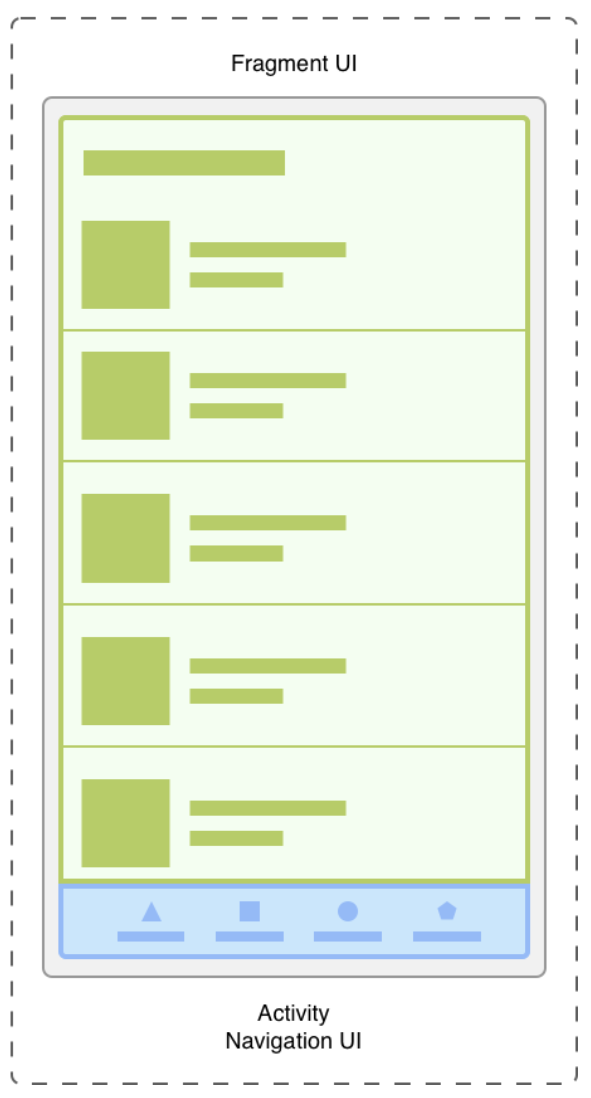
\includegraphics[width=0.4\linewidth]{tla.png}
  \caption{Der Aufbau der Applikation im Überblick.}\label{fig:tla}
\end{figure}

\subsection{Navigation}

Um die Navigation zwischen verschiedenen Ansichten einer App zu ermöglichen wird von Android die \texttt{Navigation Component}\footnote{Navigation Component. \url{https://developer.android.com/guide/navigation}} der Android-Jetpack Bibliothek bereitgestellt. Diese beinhaltet folgende Teile:

\begin{itemize}
  \item \textbf{Navigationsgraph:} Eine XML-Ressource, die alle Informationen bezüglich der Navigation an einem zentralen Ort enthält. Dazu gehören alle einzelnen Ansichten innerhalb der App, sowie die möglichen Pfade, die ein Benutzer durch Ihre App nehmen kann.
  \item \textbf{NavHost:} Ein leerer Container, welcher die Fragmente der einzelnen Navigationspfade anzeigt. Im Falle der Output App wird die Standardimplementierung \texttt{NavHostFragment} benutzt.
  \item \textbf{NavController:} Ein Objekt, das die App-Navigation innerhalb eines NavHosts verwaltet. Der NavController orchestriert das Austauschen von Zielinhalten im NavHost, wenn Benutzer durch Ihre App navigieren.
\end{itemize}

Sobald der Nutzer innerhalb der App navigiert, wird das entsprechende Fragment der Ansicht im \texttt{NavHost} dargestellt. Dabei stellt Navigationskomponente auch eine konsistente und vorhersehbare Benutzererfahrung sicher, indem sie sich an einen etablierten Satz von Prinzipien hält. Beispielsweise ermöglicht die Navigation-Komponente die Einbindung der \texttt{BottomNavigationView} mit minimalem Programmieraufwand. Unterstützt wird die Navigation durch \texttt{Safe Args}\footnote{Safe Args. \url{https://developer.android.com/guide/navigation/navigation-pass-data\#Safe-args}}, einem Gradle-Plugin, das Typsicherheit beim Navigieren und Übergeben von Daten zwischen Ansichten bietet. \Cref{fig:navigation} zeigt einen Ausschnitt der grafischen Repräsentation der Navigation innerhalb der App, wobei Pfeile den Navigations-Fluss zwischen Ansichten darstellen.   

\begin{figure}[H]
  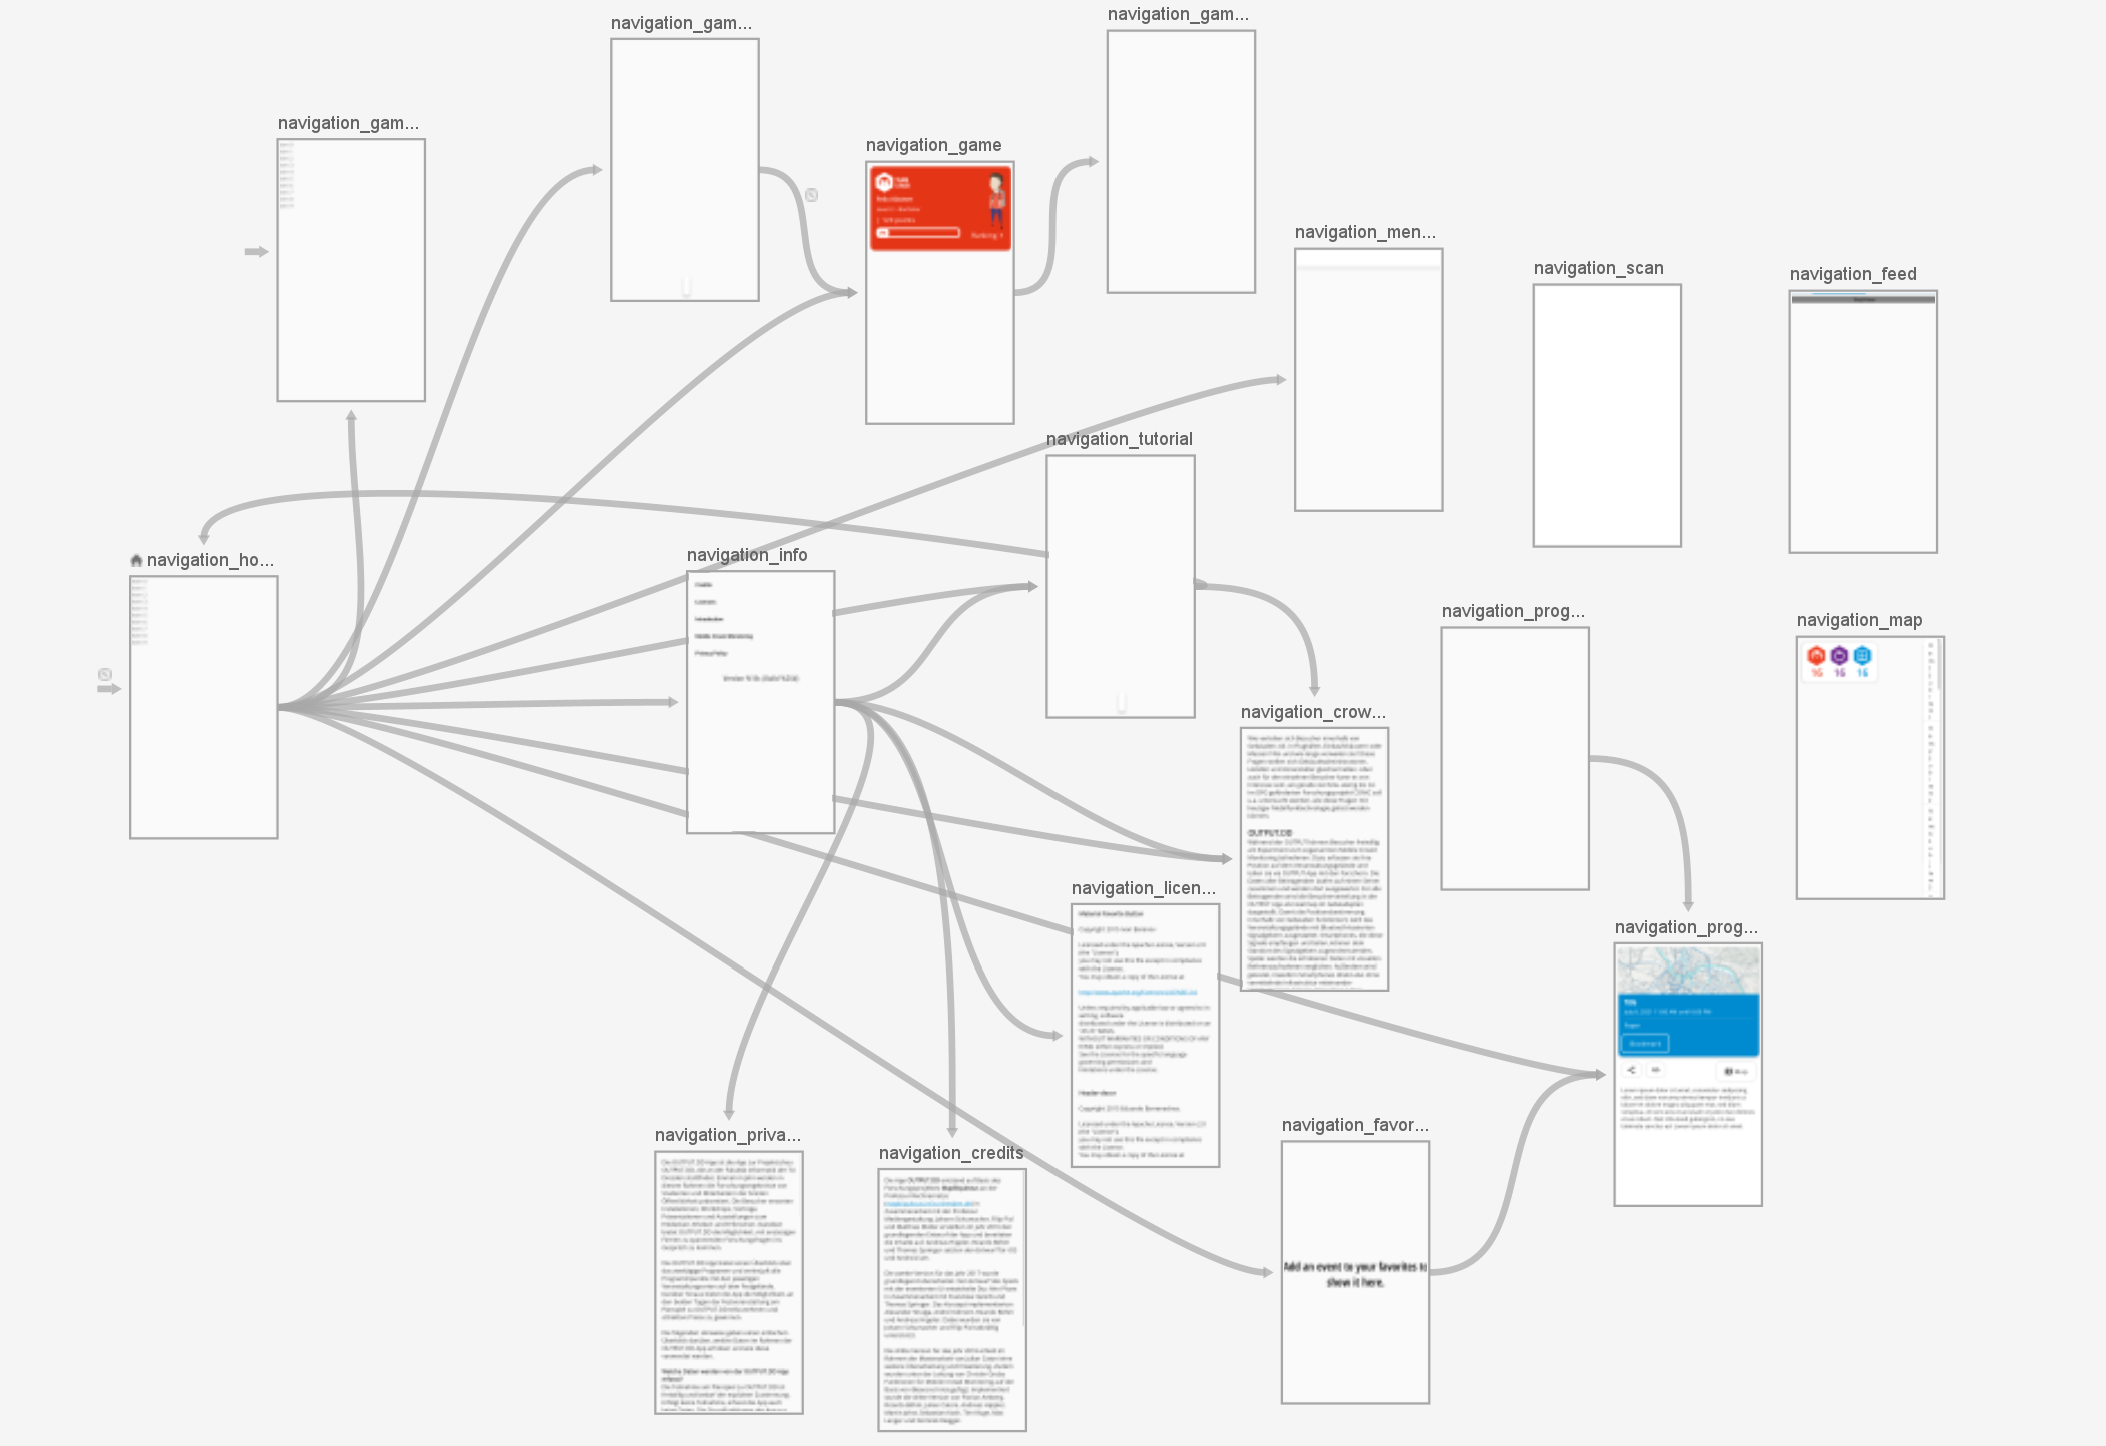
\includegraphics[width=1\linewidth]{navigation.png}
  \caption{Ausschnitt der Navigation innerhalb der OUTPUT-App.}\label{fig:navigation}
\end{figure}


\subsection{Viewbindung}\label{subsec:viewbinding}

Um einfacher mit den Ansichten interagieren zu können wird eine Technik names \texttt{Viewbinding}\footnote{Viewbinding. \url{https://developer.android.com/topic/libraries/view-binding}} verwendet. Durch die Aktivierung dieses Build-Features wird automatisch, für jede vorhandene XML-Layout-Datei eine Binding-Klasse erzeugt. Eine Instanz dieser Binding-Klasse enthält direkte Verweise auf alle Ansichten, die eine ID in dem entsprechenden Layout haben. Die Verwendung von Viewbinding erlaubt somit die objektorientierte Verwendung von Views und ersetzt gleichzeitig die Funktionalität der \texttt{findViewById}-Methode. In Bezug auf die in \Cref{lst:layout} gezeigte Layout-Datei ergibt sich die in \Cref{fig:viewbinding} dargestellte Nutzung im Quellcode.

\begin{figure}[H]
    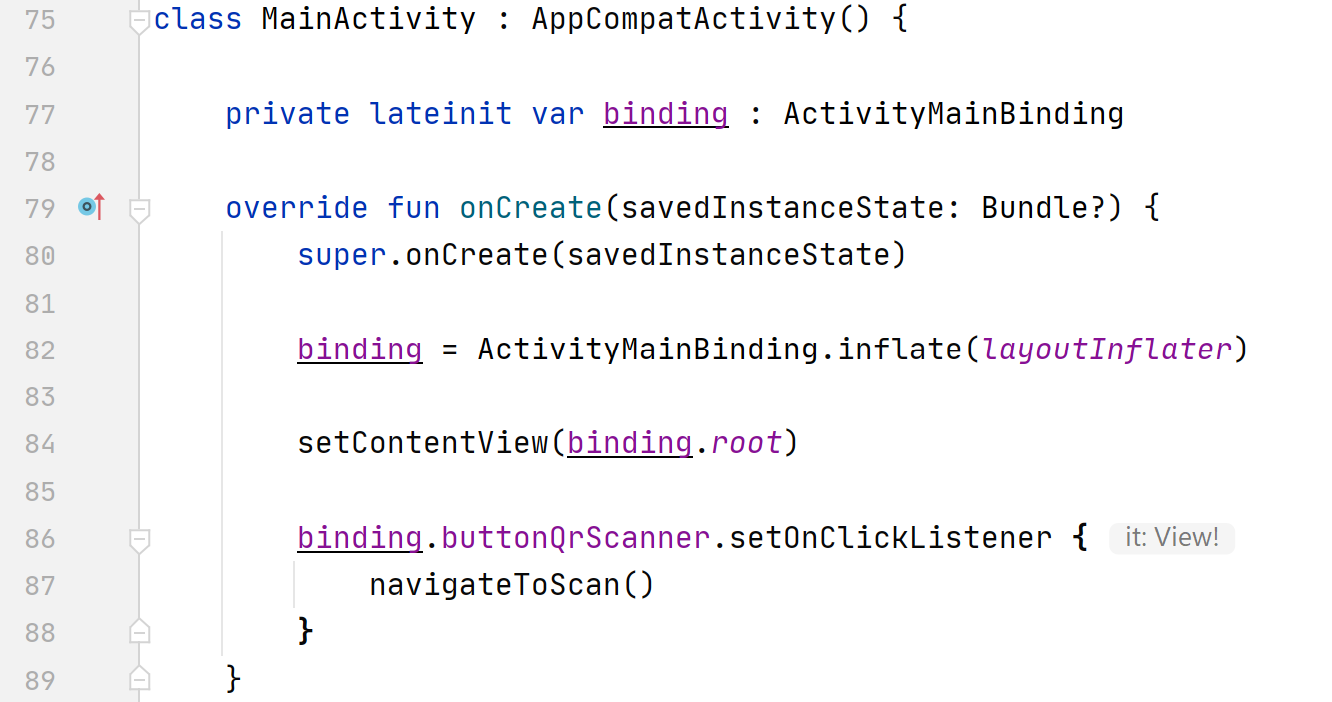
\includegraphics[width=1\linewidth]{viewbinding.png}
    \caption{Beispiel für die Nutzung von Viewbinding.}\label{fig:viewbinding}
\end{figure}

\subsection{Databinding}\label{subsec:databinding}

\texttt{Databinding}\footnote{Databinding. \url{https://developer.android.com/topic/libraries/data-binding}} ermöglicht es UI-Komponenten in Layouts an Datenquellen in der App zu binden, indem sie ein deklaratives Format verwenden. Durch die Verknüpfung von Views mit entsprechenden Daten-Variablen können programmatische Aufrufe im Quellcode reduziert werden. Dies führt nicht nur dazu, dass der Code leichter zu pflegen ist, sondern kann auch die Leistung der App verbessern und helfen, Memory-Leaks und Null-Pointer-Exceptions zu vermeiden. Äquivalent zum Fall von Viewbinding werden entsprechende Binding-Klassen automatisch generiert. Im Folgenden werden Variablen innerhalb eines \texttt{data} Blocks im XML-Layout definiert. Diese können anschließend genutzt werden, um die Attribute der Views zu konfigurieren. Die Abbildung der Daten kann sowohl \textbf{unidirektional} als auch \textbf{bidirektional} erfolgen. Die Zuweisung von Variablen erfolgt dabei einmalig zum Zeitpunkt der Initialisierung der View. Sobald sich nun die zugrunde liegenden Daten ändern, wird die View automatisch aktualisiert und erneut gerendert. \Cref{lst:databinding} zeigt die Verwendung von Databinding am Beispiel einer Trophäe in der Spielansicht. Die resultierende Ansicht ist in \Cref{fig:databinding} gezeigt.

\begin{figure}[H]
    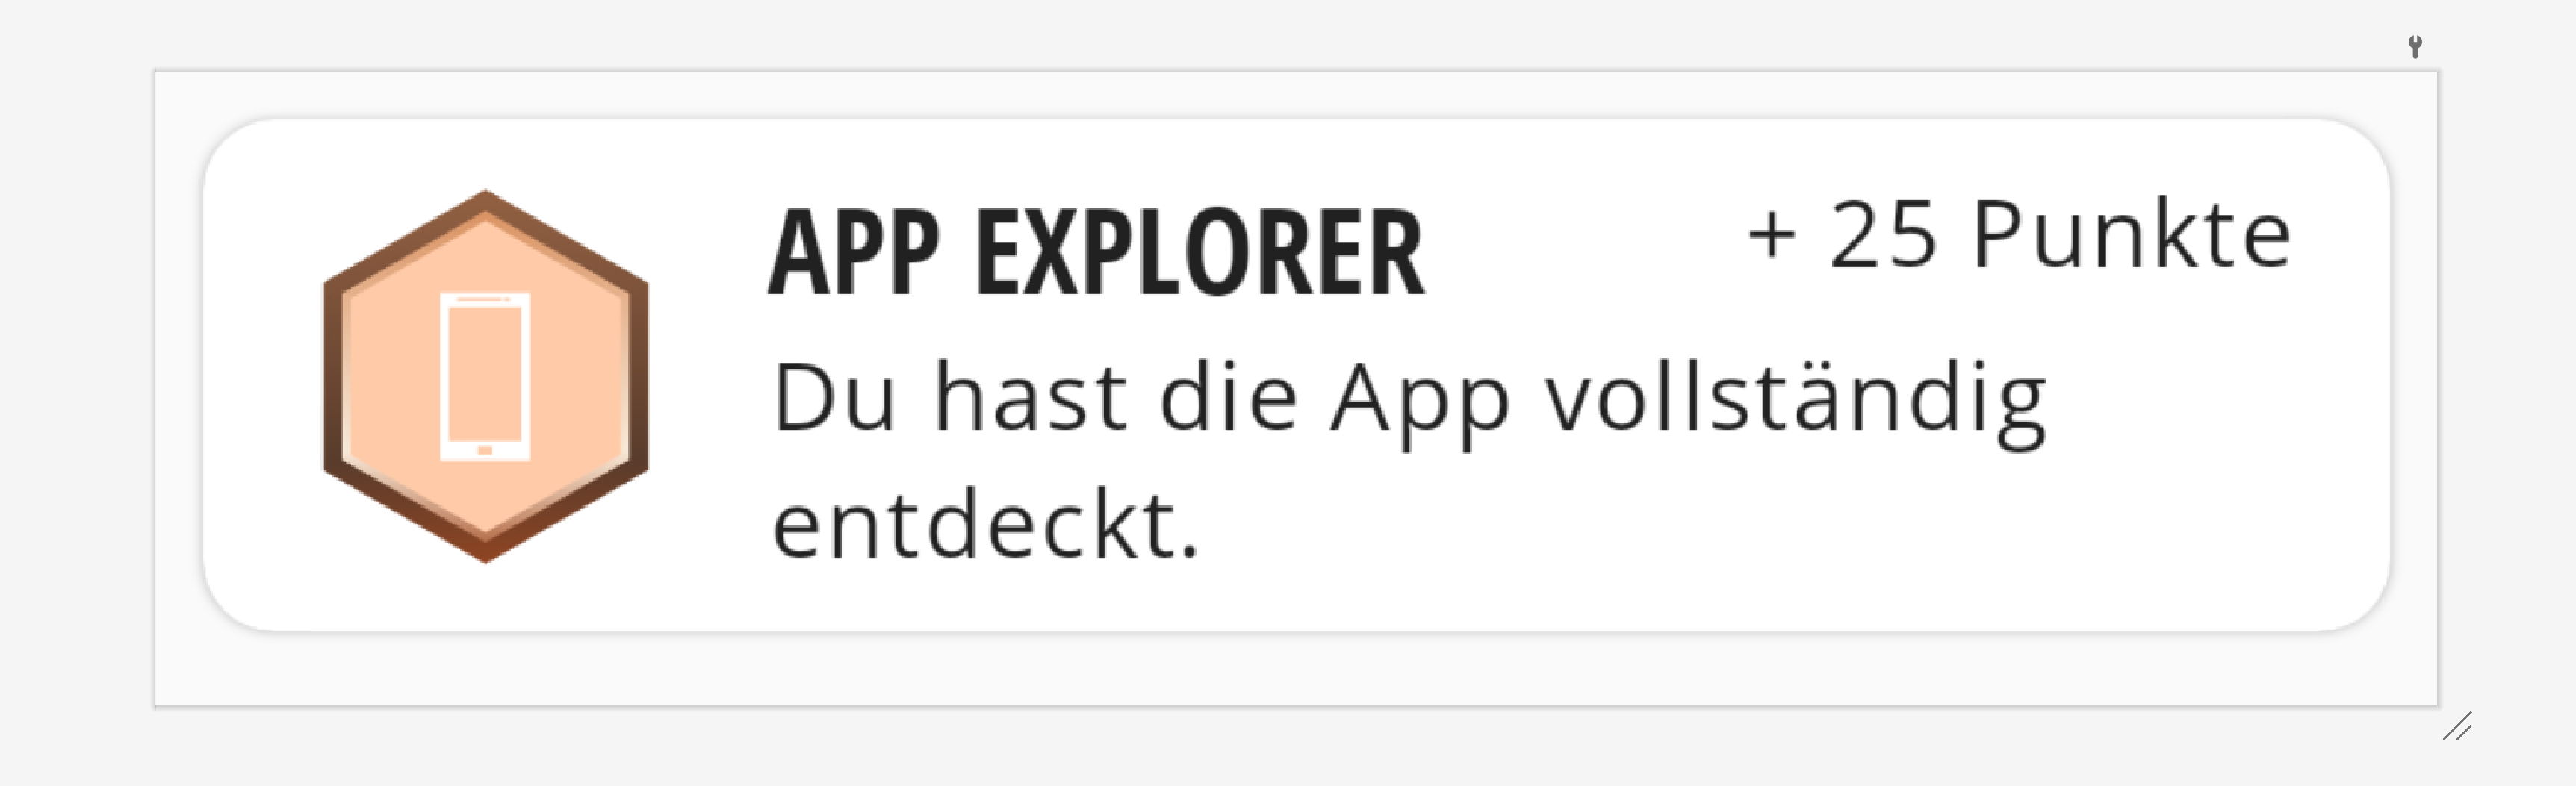
\includegraphics[width=1\linewidth]{databinding.png}
    \caption{Darstellung einer Trophäe in der Spielansicht}\label{fig:databinding}
\end{figure}

\begin{lstlisting}[language=XML, caption={Databinding am Beispiel einer Trophäe in der Spielansicht.}, label={lst:databinding}]
<layout 
    xmlns:android="http://schemas.android.com/apk/res/android"
    xmlns:app="http://schemas.android.com/apk/res-auto">
    <data>
        <variable
            name="achieved"
            type="java.lang.Boolean"/>
        <variable
            name="viewModel"
            type="de.outputdd.database.models.shared.trophy.Trophy" />
    </data>
    <com.google.android.material.card.MaterialCardView ...>
        <androidx.constraintlayout.widget.ConstraintLayout ...>

            <ImageView 
                ... 
                app:bitmap="@{viewModel.icon}"/>

            <TextView
                ...
                android:text="@{viewModel.title}"
                android:enabled="@{achieved}" />

            <TextView
                ...
                android:text="@{String.format("+ %s", viewModel.points)}"
                android:enabled="@{achieved}" />

            <TextView
                ...
                android:text="@{viewModel.details}"
                android:enabled="@{achieved}" />

        </androidx.constraintlayout.widget.ConstraintLayout>
    </com.google.android.material.card.MaterialCardView>
</layout>
\end{lstlisting}

\newpage

\section{Datenfluss- und Architektur-Patterns}

Es werden verschiedene Patterns vorgestellt, die sich im Implementationskonzept wiederfinden und auch Bestandteil der zukünftigen Entwicklung sein sollen. Diese spiegeln ebenso die Prinzipien von Android wieder und sind zentraler Bestandteil der App.

\subsection{View-Model-ViewModel-Pattern}

\textbf{Model-View-ViewModel (MVVM)} ist eine Variante des bekannten Model-View-Presenter (MVP) Entwurfsmusters. Das Ziel dieses Architektur-Patterns ist die Trennung von Darstellung und Logik der Benutzeroberfläche. Die Bestandteile des Patterns sind:

\begin{itemize}
    \item \textbf{Model:} Eine Instanz welche die Daten der Anwendungsdomäne enthält. Diese Objekte haben keinen direkten Zusammenhang zur View, sondern repräsentieren Datenbank-Objekte im Kontext der Anwendung.
    \item \textbf{View:} Die Repräsentation einer Ansicht, ohne jegliche Anwendungslogik.
    \item \textbf{ViewModel:} Die Schnittstelle zwischen den Daten im Anwendungskontext und der Repräsentation. Viewmodels stellen die Daten der Models als Datenfluss für die View bereit. 
\end{itemize}

\Cref{fig:mvvm} zeigt den Aufbau des MVVM-Patterns. Bekannte CRUD-Operationen auf den Daten werden dabei durch das Viewmodel ausgeführt. In den meisten Fällen verfügt das Model über Mechanismen um gezielt auf Änderungen der Daten reagieren zu können. Die Daten können anschließend vom ViewModel als Datenfluss für die View bereitgestellt werden. View und ViewModel verfügen über eine unidirektionale oder bidirektionale Bindung, bei welcher die View die Daten sowie Methoden des Viewmodels referenziert. Gleichzeitig kann ein gegebenes ViewModel für mehrere Views eingesetzt werden.

\begin{figure}[H]
    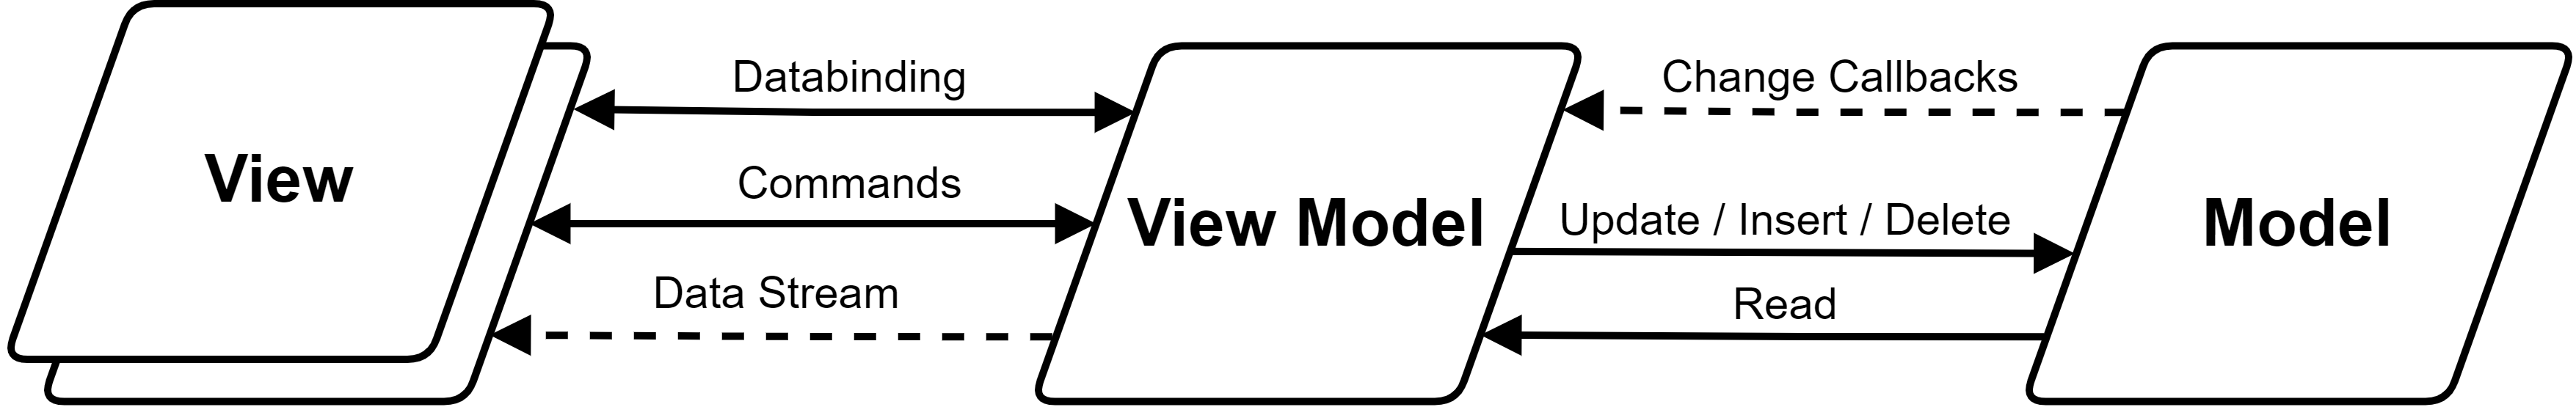
\includegraphics[width=1\linewidth]{mvvm.png}
    \caption{Aufbau des Model-View-ViewModel-Pattern.}\label{fig:mvvm}
\end{figure}

\newpage

\subsection{Observer-Pattern}\label{sub:observer}

Das \textbf{Observer-Pattern} ist ein weiteres Entwurfsmuster, welches in der Android-Entwicklung eine zentrale Rolle spielt. Es gehört zur Kategorie der Verhaltensmuster und dient zur Weitergabe von Änderungen an abhängige Datenstrukturen. Damit lassen sich Ereignis-basierte Abläufe programmieren. In der für die Android-Entwicklung üblichen Variante des Observer-Patterns, informiert ein Objekt (genannt \texttt{Subjekt}) alle  abhängigen Objekte (genannt \texttt{Observer}) von Änderungen und überträgt dabei jeweils eine aktuelle Kopie der Daten als Parameter. Der Ablauf ist in \Cref{fig:observer} gezeigt. Diese Form wird auch \texttt{Push-Update Observer} genannt. 

\begin{figure}[H]
    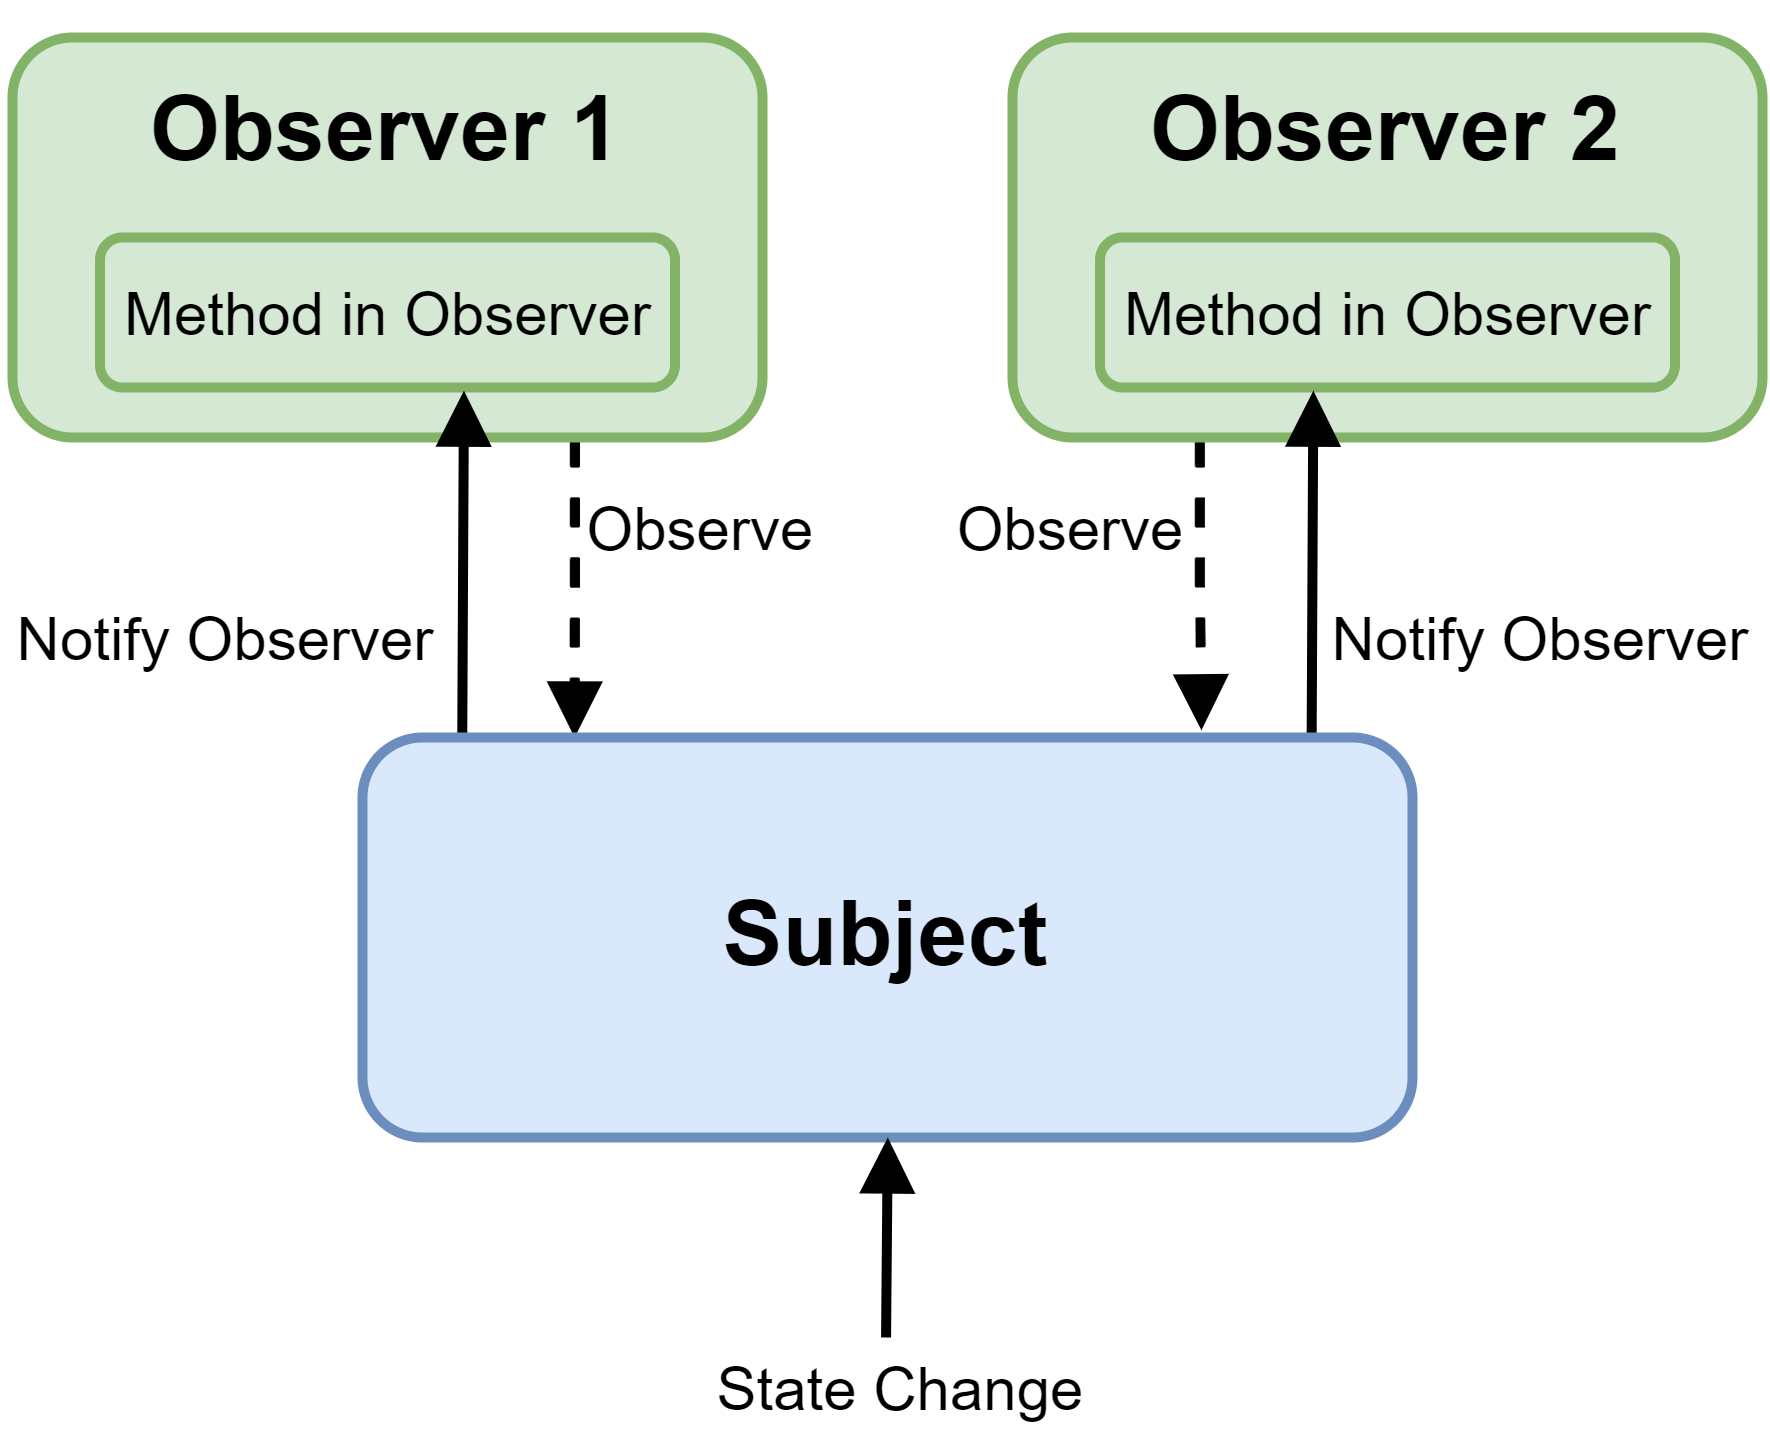
\includegraphics[width=0.65\linewidth]{observer.png}
    \caption{Aufbau des Observer-Pattern.}\label{fig:observer}
\end{figure}

\subsection{Mediator-Pattern}

Wie auch das \hyperref[sub:observer]{Observer-Pattern} zählt das \texttt{Mediator-Pattern} zu der Klasse von Verhaltensmustern. Das Mediator-Pattern richtet sich dabei an den Informationsaustausch zwischen Objekten. Die Kommunikation findet mittels eines sogenannten \texttt{Mediator}-Objekts statt, welches als Schnittstelle zwischen den beteiligten Objekten dient. Dadurch kann das kooperative Verhalten zentral verwaltet werden, wobei die Implementierung des \texttt{Mediator} unabhängig der beteiligten Objekte erfolgen kann. Somit kann eine lose Kopplung geschaffen werden, was zugleich die Komplexität der beteiligten Objekte mindert. 


\subsection{Delegation-Pattern}\label{subsec:delegation}

Das \texttt{Delegation-Pattern} ist ein strukturelles Entwurfsmuster, welches die Bildung von Objekten erleichtert und damit als Alternative zur Vererbung die Wiederverwendung von Implementationen erlaubt. Das Prinzip des Patterns beruht auf der Weitergabe von Aufrufen (\enquote{Delegation}) an ein weiteres Objekt. Die Auswertung des Zugriffs geschieht im Falle von \texttt{Delegation} im Kontext des initialen Objektes. Damit grenzt sich das Prinzip von \texttt{Delegation} klar gegenüber dem Prinzip von \texttt{Forwarding} ab, wobei die Auswertung des Zugriffes im Kontext des Objektes geschieht, an welches delegiert wurde. Das Pattern wird nativ von der Programmiersprache \hyperref[sec:kotlin]{Kotlin} unterstützt und kann somit ohne weiteres direkt als Element der Programmiersprache verwendet werden. Kotlin unterstützt dabei sowohl die Delegation von Interfaces\footnote{Delegation. \url{https://kotlinlang.org/docs/delegation}} sowie die Delegation von einzelnen Eigenschaften\footnote{Delegated Properties. \url{https://kotlinlang.org/docs/delegated-properties.html}}.
